\errorcontextlines=200
%\documentclass[10pt]{book}
%\usepackage[whole]{bxcjkjatype}
%\documentclass[pdflatex,a5paper,10pt]{bxjsbook}
\documentclass[platex,dvipdfmx,a5paper,10pt]{bxjsbook}
\usepackage{framed}
\setlength{\FrameSep}{0mm}

% For Japanese index
\usepackage{imakeidx}
\makeindex
\makeindex[name=ja, title={日本語牽引}]
\newcommand{\ejindex}[2]{\index{#1}\index[ja]{#2}}

%\makeindex
%\usepackage{showidx}
% mark overful hboxes
%\overfullrule=5mm
\usepackage{kpfonts}

\newcommand{\eq}{=}

%\usepackage[nott]{kpfonts}
%\SetMathAlphabet{\mathtt}{normal}{OT1}{\ttdefault}{m}{n}
%\SetMathAlphabet{\mathtt}{bold}{OT1}{\ttdefault}{m}{n}

%\usepackage[math]{iwona}
%\SetMathAlphabet{\mathtt}{iwona}{OT1}{\ttdefault}{m}{n}
%\usepackage[T1]{fontenc}

\usepackage{amsopn}
\usepackage{amsmath}
\usepackage{amsthm}
\usepackage{url}
\usepackage[dvipdfmx]{graphicx}
\usepackage{datetime}
\usepackage{amsfonts}
\usepackage{graphicx}
\usepackage{threeparttable}
\usepackage{wasysym}
\usepackage{emptypage}
\usepackage{titling}
\usepackage{array}
%\usepackage{calc}


%\usepackage[mathlines]{lineno}
%\linenumbers
%\DeclareGraphicsExtensions{.pdf,.eps}

% Leave this here - it gets substituted with language specific stuff
%HEADCOMMAND

\allowdisplaybreaks[1]  % for ams math align environments

\hyphenation{Array-Stack}
\hyphenation{Fast-Array-Stack}
\hyphenation{Array-Queue}
\hyphenation{Array-Deque}
\hyphenation{Dual-Array-Deque}
\hyphenation{Root-ish-Array-Stack}
\hyphenation{Skip-list-Set}
\hyphenation{Skip-list-List}
\hyphenation{Hash-Table}
\hyphenation{Chained-Hash-Table}
\hyphenation{Linear-Hash-Table}
\hyphenation{Red-Black-Tree}
\hyphenation{Binary-Tree}
\hyphenation{Binary-Search-Tree}
\hyphenation{Scape-goat-Tree}
\hyphenation{Count-down-Tree}
\hyphenation{Dy-na-mite-Tree}
\hyphenation{Binary-Heap}
\hyphenation{Meld-able-Heap}
\hyphenation{Java-Script}

%\usepackage{everysel}
\usepackage{pxeverysel}
\EverySelectfont{%
%\fontdimen2\font=0.4em% interword space
%\fontdimen3\font=0.2em% interword stretch
%\fontdimen4\font=0.1em% interword shrink
%\fontdimen7\font=0.1em% extra space
\hyphenchar\font=`\-% to allow hyphenation
}

\let\emph\relax % there's no \RedeclareTextFontCommand
\DeclareTextFontCommand{\emph}{\bf}

\usepackage[sf,small,raggedright]{titlesec} % formatting titles
\usepackage{etoolbox}
\makeatletter
\patchcmd{\ttlh@hang}{\parindent\z@}{\parindent\z@\leavevmode}{}{}
\patchcmd{\ttlh@hang}{\noindent}{}{}{}
\makeatother

\titlespacing*{\section}{0pt}{24pt}{14pt}
\titlespacing*{\subsection}{0pt}{14pt}{14pt}
\usepackage{relsize,fancyvrb}  % formatting pseudocode
\usepackage{ods} % Personalization and commands

%\renewcommand*{\thechapter}{\arabic{chapter}~章}
\titleformat*{\chapter}{\large\bfseries}

% These command are expanded by scripts, otherwise they should be ignored
\newcommand{\javaimport}[1]{}
\newcommand{\cppimport}[1]{}
\newcommand{\pcodeimport}[1]{}

\htmlonly{
  \newcommand{\ScaleIfNeeded}{\textwidth}
  \newcommand{\HalfScaleIfNeeded}{\textwidth}
  \newcommand{\HeightScaleIfNeeded}{\textheight}
  \newcommand{\QuarterHeightScaleIfNeeded}{.25\textheight}
  \newcommand{\FifthHeightScaleIfNeeded}{.2\textheight}
  \newcommand{\fancyhead}[2][zzz]{}
  \newcommand{\fancyfoot}[2][zzz]{}
}

% Referencing commands 
\newcommand{\chaplabel}[1]{\label{chap:#1}}
\newcommand{\Chapref}[1]{\ref{chap:#1}~章}
\newcommand{\chapref}[1]{\ref{chap:#1}~章}
\newcommand{\seclabel}[1]{\label{sec:#1}}
\newcommand{\Secref}[1]{\ref{sec:#1}~節}
\newcommand{\secref}[1]{\ref{sec:#1}~節}
\newcommand{\sref}[1]{\textsection~\ref{sec:#1}}

\newcommand{\alglabel}[1]{\label{alg:#1}}
\newcommand{\Algref}[1]{アルゴリズム~\ref{alg:#1}}
\newcommand{\algref}[1]{アルゴリズム~\ref{alg:#1}}

\newcommand{\applabel}[1]{\label{app:#1}}
\newcommand{\Appref}[1]{付録~\ref{app:#1}}
\newcommand{\appref}[1]{付録~\ref{app:#1}}

\newcommand{\tablabel}[1]{\label{tab:#1}}
\newcommand{\Tabref}[1]{表~\ref{tab:#1}}
\newcommand{\tabref}[1]{表~\ref{tab:#1}}

\newcommand{\figlabel}[1]{\label{fig:#1}}
\newcommand{\Figref}[1]{図~\ref{fig:#1}}
\newcommand{\figref}[1]{図~\ref{fig:#1}}

\newcommand{\eqlabel}[1]{\label{eq:#1}}
\newcommand{\myeqref}[1]{(\ref{eq:#1})}
\newcommand{\Eqref}[1]{式~(\ref{eq:#1})}

% Theorem-like environments
\theoremstyle{plain}
\newtheorem{thm}{定理}[chapter]
\newcommand{\thmlabel}[1]{\label{thm:#1}}
\newcommand{\thmref}[1]{定理~\ref{thm:#1}}

\newtheorem{lem}{補題}[chapter]
\newcommand{\lemlabel}[1]{\label{lem:#1}}
\newcommand{\lemref}[1]{補題~\ref{lem:#1}}

\newtheorem{cor}{系}[chapter]
\newcommand{\corlabel}[1]{\label{cor:#1}}
\newcommand{\corref}[1]{系~\ref{cor:#1}}

\theoremstyle{definition}

\newtheorem{exc}{問}[chapter] % 問題はtechnical term?
\newcommand{\exclabel}[1]{\label{exc:#1}}
\newcommand{\excref}[1]{問~\ref{exc:#1}}


\newtheorem{prp}{性質}[chapter]
\newcommand{\prplabel}[1]{\label{prp:#1}}
\newcommand{\prpref}[1]{性質~\ref{prp:#1}}


% Miscellaneous commands
\newcommand{\etal}{\emph{et al.}}
\newcommand{\voronoi}{Vorono\u\i}
\newcommand{\ceil}[1]{{\lceil #1 \rceil}}
\newcommand{\Ceil}[1]{{\left\lceil #1 \right\rceil}}
\newcommand{\floor}[1]{{\lfloor #1 \rfloor}}
\newcommand{\Floor}[1]{{\left\lfloor #1 \right\rfloor}}
\newcommand{\R}{\mathbb{R}}
\newcommand{\N}{\mathbb{N}}
\newcommand{\Z}{\mathbb{Z}}
\newcommand{\Sp}{\mathbb{S}}
\newcommand{\E}{\mathrm{E}}
\DeclareMathOperator{\ddiv}{div}

\renewcommand\proofname{\bf 証明}


\usepackage{ods-colors}

\usepackage{tikz,gnuplot-lua-tikz}

\usepackage[bookmarks]{hyperref}
\hypersetup{colorlinks=true, linkcolor=linkblue,  anchorcolor=linkblue,%
	citecolor=linkblue, filecolor=linkblue, menucolor=linkblue,%
	urlcolor=linkblue,%
    pdfauthor={Pat Morin},%
    pdftitle={Open Data Structures},%
    pdfsubject={Computer Science, Data Structures},%
    pdfkeywords={Data structures, algorithms}} 

\DeclareMathOperator{\bdiv}{div}

% Title page content
\title{Open Data Structures (in \lang) 日本語版}
\author{Pat Morin}
\date{%
Edition 0.1G\cpponly{$\beta$}\pcodeonly{$\beta$}
\htmlonly{\\ 
\includegraphics[scale=0.90909,scale=0.5]{images/cc-by}}}
%Version 0.0 pre $\alpha$: \today}

\pagenumbering{roman}

% Draft mode only - mark overfull hboxes
% \overfullrule=5pt

% For Japanese YJ
%\titleformat{\chapter}[display]
%  {\huge\headingfont}{\chaptertitlename\ \thechapter}{20pt}{\Huge}


\begin{document}


%%\AddToShipoutPicture*{\BackgroundPic}
\htmlonly{\newcommand{\thetitlepage}{
  \begin{center}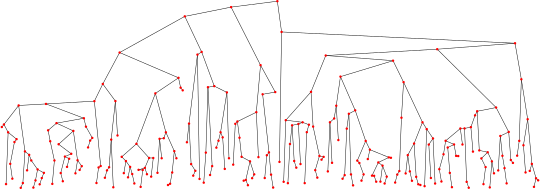
\includegraphics[scale=0.90909]{images/tree3-thick}\end{center}
  \maketitle
}}
\thetitlepage

\cleardoublepage
%
%% blank page behind title page
%\ \thispagestyle{empty}\newpage
%
%\setcounter{page}{1}
%\chapter*{Acknowledgments}
\addcontentsline{toc}{chapter}{Acknowledgments}

I am grateful to Nima~Hoda, who spent a summer tirelessly proofreading
many of the chapters in this book; to the students in the Fall 2011
offering of COMP2402/2002, who put up with the first draft of this book
and spotted many typographic, grammatical, and factual errors; and to
Morgan~Tunzelmann at Athabasca University Press, for patiently editing
several near-final drafts.

%\ \thispagestyle{empty}\newpage
%\cpponly{\cpponly{
\chapter*{Preface to the C++ Edition}
\addcontentsline{toc}{chapter}{Preface to the C++ Edition}

This book is intended to teach the design and analysis of basic data
structures and their implementation in an object-oriented language.
In this edition, the language happens to be C++.

This book is not intended to act as an introduction to the C++ programming
language.  Readers of this book need only be familiar with the basic
syntax of C++ and similar languages.  Those wishing to work with the
accompanying source code should have some experience programming in C++.

This book is also not intended as an introduction to the C++ Standard
Template Library or the generic programming paradigm that the STL
embodies.  This book describes implementations of several different data
structures, many of which are used in implementations of the STL. The
contents of this book may help an STL programmer understand how some of
the STL data structures are implemented and why these implementations
are efficient.
}

%\ \thispagestyle{empty}\newpage
%}

% Use 14pt between lines
\setlength{\baselineskip}{14pt}


%\begin{titlepage}
%\maketitle
%\end{titlepage}

%\pagestyle{empty}
%half title page
%\newpage
%
%series page
%\newpage
%
%title page
%\newpage

\addtocontents{toc}{\protect\thispagestyle{empty}} % get rid of page number
\tableofcontents
\cleardoublepage

\fancyhead[RO,LE]{} % disable section numbers, for now
\pagestyle{fancy}
\chapter*{訳者まえがき}
\addcontentsline{toc}{chapter}{訳者まえがき}

%\chapter*{なぜ翻訳するのか}
%\addcontentsline{toc}{chapter}{なぜ翻訳するのか}
本書は、``Open Data Structures''という本を日本語に訳したものだ。

訳者らも含め、日本語での生活に慣れていれば、英語よりも日本語で書かれた書籍のほうがだいぶスムーズに読めるだろう。
とはいえ、これは訳者の個人的な意見だが、専門書を選ぶときにはついつい翻訳されたものを避けてしまう。
品質のばらつきが大きかったり、むしろ読みにくかったりすることが多いと感じるからだ。

しかし、この教科書は入門書である。
前提とする知識は、高校で習う数学の一部だけである(もちろん、簡単なプログラミング経験があったほうが内容に実感が持ててありがたみがわかり、楽しく読めるのは間違いない)。
本書のような入門書が日本語で読めるようになっているほうが、分野の裾野を広げ、楽しくプログラムを書ける人や効率的なプログラムが書ける人を増やしてくれるだろう。

母国語で大学レベルの教科書が読める国は多くないといわれる。
より専門的な内容はもっぱら英語で読むことになるのだから、さっさと崖から突き落としたほうがいいという意見も聞く。
大学生になっても日本語で教科書が読めるという恵まれた環境が、日本人の英語アレルギーを支えている可能性もあるだろう。
訳者自身も、「英語を読む」ところまでは受験勉強で慣れたものの、大学に入った頃はまだ「英語で読む」ことに抵抗があった。
そのような抵抗を可及的速やかに取り除き、「英語で読む」ことに慣れるのは、アクセスできる知識を押し広げるために極めて重要である。

しかし、この教科書は専門分野への橋渡しの、その初っ端に位置するものだ。
前提として要求される知識も多くない。それが、英語であるばかりに対象読者が大きく制限されているとしたら残念なことである。
母国語でこのような入門書が読める、少なくともその選択肢があるのは望ましいことであろう。

この教科書は、300ページ程度ながら、丁寧にゆっくりと、それでいて実用的な題材が扱われている。
この分野には本書より本格的な教科書も数多く出版されており、いくつかは翻訳もされている。
訳者自身がいまでも折にふれ読み返すような、素晴らしい内容のものもある。
例えば、``Algorithm Design''\footnote{Kleinberg, Jon, and Eva Tardos. Algorithm design. Pearson Education, 2006.}と``Introduction to Algorithms''\footnote{Cormen, Thomas H., et al. Introduction to algorithms. MIT press, 2009.}の二冊は翻訳も良い。
とはいえ、いずれも大判で1000ページ程度、価格は1万円程度という本であり、気軽に読めるものではない。
こうした、より専門的な書籍への橋渡しであるこの教科書を日本語で、かつ無料でも読めるようにすることが、この翻訳プロジェクトの目的である。

%堀江 慧(@spinute)

\section*{本書の読み方}
\addcontentsline{toc}{section}{本書の読み方}

本書『みんなのデータ構造』の想定読者は、初学者からベテランのエンジニアまで、データ構造にかかわるすべての人である。
訳者らが読者に伝えたいことは次の3つである。

\begin{enumerate}
\item {\bf ソフトウェアのほとんどはシンプルなデータ構造の組み合わせでできている。} \\
本書で紹介するデータ構造はシンプルなものである。よくある誤解は、これらのデータ構造は理論上のものであり、実際のソフトウェアはもっと複雑なデータ構造を使っているというものだ。これはまったくの間違いである。OSやブラウザなどの複雑なソフトウェアも、その実、シンプルなデータ構造の組み合わせでできている。本書で紹介するデータ構造が理解できれば、多くのソフトウェアの骨子が理解できるようになるだろう。言い換えれば、本書が紹介するのはおもちゃのデータ構造ではなく、現実のプログラムの中で実際に使われているデータ構造である。% spinute: まえがきなので、高校生をちょっと意識して、実務という表現を避けました

\item {\bf 本書の内容がだいたいわかるようになれば良いエンジニアになれる。} \\
ソフトウェアのほとんどが基本的なデータ構造の組み合わせでできているということは、基本的なデータ構造を理解すれば、新しいソフトウェアをデザインし、既存のソフトウェアの改良ができるようになるということである。

\item {\bf わからない部分は飛ばしてもよい。} \\
本書には数学の理解を必要とする解析がある。
理解できない部分があったら読み飛ばしても差し支えない。
あるいは、詳しい知り合いや翻訳者、著者に質問するべきである。
理解できない原因は読み手にはなく、書き手が問題だと考えるべきである。
いずれにせよ、わからない箇所があったらそこで立ち止まるのではなく、そのまま先に進めるところまで進んでみることを勧めたい。

\end{enumerate}

上記の2つめの点に関し、訳者らは、本書で扱われているデータ構造のうち実用上極めて重要な項目とそうではない項目とを明確に区別しておくことが有益だと考えた。
以下に列挙する項目は、本書の中でも特に重要であると、訳者の3人全員が判断したものだ。
学術研究やプログラマの実務で頻繁に登場する内容なので、すべての学習者が深く理解しておくことが望ましいだろう。
%これらは、この本を教科書として指定した約4ヶ月の講義\footnote{2017年度の東京大学学際科学科総合情報学コースにおける学部生向け講義「情報数理科学2」。正確には、幅優先探索と深さ優先探索については別の授業で扱われる。https://lecture.ecc.u-tokyo.ac.jp/~ktanaka/mis2-2017/index.html}で扱われる事項の部分集合になっている。
% YJ: この情報は必要か?もし必要ならば駒場だけでなく様々な大学のカリキュラムを調査するべきでは。大学の授業に言及することで高校生以下の学生が、自分にはまだ難しい内容だと勘違いしないだろうか。
%% spinute: 読者目線ではIDSが出てくる必要を感じなかったので削りました。

\begin{itemize}
  % \item 第1章: (数学的基礎の確認の章のため、該当なし)
  \item 第2章: ArrayStack、ArrayQueue、ArrayDeque
  \item 第3章: SLList、DLList
  % \item 第4章: (該当なし)
  \item 第5章: ChainedHashTable
  \item 第6章: BinaryTree、BinarySearchTree
  % \item 第7章: (該当なし)
  % \item 第8章: (該当なし)
  \item 第9章: RedBlackTree(\secref{left-redblack}から\secref{redblack-elem-remove}は複雑なので読み飛ばしてよい)
  \item 第10章: BinaryHeap
  \item 第11章: MergeSort、QuickSort
  \item 第12章: 幅優先探索、深さ優先探索
\end{itemize}

上記に列挙しなかった、ややマイナーなデータ構造にも、別の意味で学ぶ価値はある。
マイナーゆえに直接役立つ機会は少ないかもしれないが、その背後にあるアイデアやその解析手法は多くの場面で読者の助けになるはずだ(単純に知的な面白さのある話題も多い)。
どの章を重点的に読むか、興味に応じて適宜調整してほしい。
% YJ: Introduction to Algorithm, Algorithm Designなどに言及する?

本書の日本語版のプロジェクトページ\footnote {\url{https://sites.google.com/view/open-data-structures-ja}}には、本書の他言語版やプロジェクトに関する情報がある。
本書の日本語版のソースコードはGitHub\footnote {\url{https://github.com/spinute/ods}}にある。

\section*{訳者謝辞}
\addcontentsline{toc}{section}{訳者謝辞}

まずなにより、本書の原著者であるPat Morinに感謝する。
Patは、Open Data Structuresを立ち上げ、再配布、改変、販売を許容するライセンスで公開してくれた。
本書の日本語訳プロジェクトは、Patが書いた``My hope is that, by doing things this way, this book will continue to be a useful textbook long after my interest in the project, or my pulse, (whichever comes first) has waned.''という一文に惹かれて始めたものである。
Patは、翻訳、クラウドファンディング、出版のいずれの相談にも前向きな返事をくれ、また、そのたびにencourageしてくれた。

本プロジェクトでは、成果物の品質を高めるために、書籍をプロの編集者にレビューしてもらうための資金を募るクラウドファンディングを行った。
このクラウドファンディングに参加していただいた皆様にも感謝を捧げたい。
次の団体、企業、個人をはじめとしてたくさんの方々からご支援いただいた(敬称略)。 % 掲載不要とした人も沢山おり、その方々への感謝もしたい
\begin{itemize}
\item 斉藤淳(J PREP)、東京大学瀧本哲史ゼミ、株式会社バオバブ、有限会社コンセントレーション
\item 上田真道、長谷川悠斗、赤野健悟、石田修平、瓜生英尚、Kiyotaka Saito、桑田誠、小林元、石畠正和、t2nis、永浦 尊信、wtokuno、katsyoshi、ysaito、前原貴憲、髙木正弘、Yoshinari Takaoka(a.k.a mumumu)、T.Miyazawa、佐藤怜、田中哲朗、Masashi Fujiwara、雪村あおい、Tetsuya Yamazaki、永本、武平佑太、Yamachan0928、新海息吹、Daiki Sugiyama、早瀬元、山口駿人、長谷川拓也、okue、飛田晃介、大坂直人、松林祐、若杉武史、Hideki Hamada、落合哲治、鈴木 研吾、redfield920、山崎宏宇、宮田潔志
\end{itemize}

皆様のおかげで本書のソースコードを原著と同様にCreative Commons Attributionライセンスで公開できた。
また、本書の原稿は出版社でのレビューを経て、かなり読みやすくなった。
さらには、余剰金で情報オリンピックの日本代表選抜に参加する学生に、書籍を献本することも計画している。
この本が多くの人に読まれ、日本のプログラミングや情報科学を支える人たちの一助となることを強く願っている。

ラムダノート社の鹿野さん、高尾さんにもこの場をお借りしてお礼を申し上げたい。
ラムダノートは 2015 年に設立された新進気鋭の技術出版社である。
このプロジェクトのクラウドファンディングを見て、本書の編集作業を破格の条件で引き受けてくださった。
また、出版の企画を持ちかけ、書籍としての完成度を高めるための惜しみない援助をしてくださった
\footnote{本書の原稿はオープンソースであり、GitHubで公開されている。プロの編集者の手にかかると書籍がどう変貌するのかに興味がある読者は、2018年1月時点の原稿と、いまのこの本を比較してみると感動するのではないかと思う。}。

% 「書籍」と「本」が紛らわしい <- spinute: 書籍はphysical bookという気持ちで使っていたような(オレオレ用法な気もするし、紛らわしいのは事実...)
この翻訳プロジェクトは、2017年の春に堀江が個人的に始めたものである。
その時点では、ただ日本語訳を作成することしか考えていなかった。
その後、試しに陣内に原稿を見てもらったときに「この本は価値がある」と言われたことを受け、より多くの読者に読んでもらうためクラウドファンディングを企画した。
また、陣内は共訳者として本書のすべての章をレビューし、プロジェクト自体の運営にも携わってくれた。
一目置く陣内からの後押しは、GitHubの隅に眠っていたかもしれない本書の運命を変えた。
堀江、陣内とは違った角度から問題を解決する能力のある田中も、本書のレビューとプロジェクトの運営との両面で協力してくれた。
クラウドファンディングでの成功には人望の厚い田中の協力が欠かせなかった。
また、多くの修正や訳注を加えて本書をより理解しやすくしてくれた。
大学を卒業した後も、またこの二人と仕事ができて嬉しい。

\noindent\hspace*{2em}
2018年7月

\hfill 堀江 慧(@spinute)

\chapter*{Acknowledgments}
\addcontentsline{toc}{chapter}{Acknowledgments}

I am grateful to Nima~Hoda, who spent a summer tirelessly proofreading
many of the chapters in this book; to the students in the Fall 2011
offering of COMP2402/2002, who put up with the first draft of this book
and spotted many typographic, grammatical, and factual errors; and to
Morgan~Tunzelmann at Athabasca University Press, for patiently editing
several near-final drafts.

\thispagestyle{empty}
\cleardoublepage

\fancyhead[CE]{\small Why This Book?} % chapter title, left center
\chapter*{なぜこの本を書いたのか}
% TALK: Why This Book? はどういう意図か?例:「なぜこの本はあるのか?」「なぜこの本を筆者が書いたのか?」「なぜこの本を読者が読むのか?」(内容的に最後のものではなさそう。)
\addcontentsline{toc}{chapter}{なぜこの本を書いたのか}

いろいろなデータ構造の入門書がある。出来の良いものもある。ほとんどはタダではないので、コンピュータサイエンスを学ぶ学部生はデータ構造の本にお金を払うだろう。

オンラインで公開されているデータ構造の本もある。名作もあるのだが古くなってきているものが多い。ほとんどは著者や出版社が更新をやめるときに無料になったものである。これらの本は次の理由からふつうは内容を更新できない。(1)著者または出版社が著作権を持っていて、いずれかの許可を得られないため。(2)書籍の\emph{ソースコード}が提供されていないため。つまり、本のWord、WordPerfect、FrameMaker、または\LaTeX{}ソースコードが手に入らない、またはそれを扱えるソフトウェアのバージョンが手に入らないため。

このプロジェクトの目標は、コンピュータサイエンスを専攻する学部生が負担するデータ構造の入門書代をゼロにすることだ。そのため、オープンソース\ejindex{Open Source}{おーぷんそーす@オープンソース}のソフトウェアプロジェクトのようにこの本を作ることにした。この本の\LaTeX{}ソース、\lang{}ソース、およびビルドスクリプトを、著者のWebサイト\footnote {\url{http://opendatastructures.org} [訳注]日本語版のWebサイトは\url{https://sites.google.com/view/open-data-structures-ja}}、あるいは信頼できるソースコード管理サイト\footnote {\url{https://github.com/patmorin/ods} [訳注]日本語版のソースコードは\url{https://github.com/spinute/ods}}からダウンロードできる。

% TODO: 書籍版は Creative Commons ではないので、書籍版のこの部分ではそのことを注記したほうがよさそう
ソースコードはCreative Commons Attributionライセンスで公開されている。つまり、誰でも自由にコピー、配布、送信してよい。内容を取り入れて別の何かを作ってもよい。そしてそれを商業的に利用してもよい。唯一の条件は\emph{帰属の表示(attribution)}である。つまり、派生した作品が\url{opendatastructures.org}のコードやテキストを含むことを明記しなければならない。

ソースコード管理システム\texttt{git}\index{git@\texttt{git}}による修正を通して、誰でも本書に貢献できる。本のソースをフォークして、別のバージョンを作ってもよい(例えば、別のプログラミング言語を題材にした版を作れる)。こうしたやり方で、私のやる気や興味が衰えたあとでも、この本が役立つものであり続けることを望んでいる。

\hfill Pat Morin

\cleardoublepage

\cpponly{
  \cpponly{
\chapter*{Preface to the C++ Edition}
\addcontentsline{toc}{chapter}{Preface to the C++ Edition}

This book is intended to teach the design and analysis of basic data
structures and their implementation in an object-oriented language.
In this edition, the language happens to be C++.

This book is not intended to act as an introduction to the C++ programming
language.  Readers of this book need only be familiar with the basic
syntax of C++ and similar languages.  Those wishing to work with the
accompanying source code should have some experience programming in C++.

This book is also not intended as an introduction to the C++ Standard
Template Library or the generic programming paradigm that the STL
embodies.  This book describes implementations of several different data
structures, many of which are used in implementations of the STL. The
contents of this book may help an STL programmer understand how some of
the STL data structures are implemented and why these implementations
are efficient.
}

  \cleardoublepage
}

\fancyhead[CE]{\small\nouppercase{\leftmark}} % chapter title, left center
\fancyhead[CO]{\small\rightmarktitle} % section title, right center
\fancyhead[RO,LE]{\small\rightmarksection}

%% Include all the chapters one at a time

\include{intro-lang}
\include{arrays-lang}
\include{linkedlists-lang}
\include{skiplists-lang}
\include{hashing-lang}
\include{binarytrees-lang}
\include{rbs-lang}
\include{scapegoat-lang}
\include{redblack-lang}
\include{heaps-lang}
\include{sorting-lang}
\include{graphs-lang}
\include{integers-lang}
\include{btree-lang}

%% Turn off section numbers for remainder of document
\fancyhead[RO]{} % section number on the outside
\fancyhead[LE]{} % section number on the outside
\renewcommand{\chaptermark}[1]{\markboth{#1}{}} 
\renewcommand{\sectionmark}[1]{\markright{#1}} 
\fancyhead[CO]{\small\nouppercase\rightmark}

\cleardoublepage
\addcontentsline{toc}{chapter}{Bibliography}
\bibliographystyle{abbrvurl}
\bibliography{ods,odsproc}

\cleardoublepage
\addcontentsline{toc}{chapter}{Index}
\printindex
\printindex[ja]

\end{document}

